\documentclass[german,11pt,a4paper]{netforms}

\usepackage[T1]{fontenc}
\usepackage[utf8]{inputenc}
\usepackage{geometry}
\usetikzlibrary{calc}


% Alle Konfigurationsbefehle sind optional. Fehlende Befehle fueheren einfach
% zu "blank forms".

% Typ der Arbeit/Einstellung. Gueltige Argumente sind:
% bachelor,master,diplom,idp,gr,hiwi,other
% Falls 'other' gewaehlt wird, kann als optionales Argument eine spezielle Art
% von Abschlussarbeit angegeben werden, z.B. \type[Sklave]{other}. Andernfalls
% wird 'Other' als Standardbeschreibung gesetzt.
\type{bachelor}

% Informationen ueber den Studenten. Sollte selbsterklaerend sein.
\anrede{Herr}
\nachname{nachname}
\vorname{vorname}
\matrikel{matrikel}
\sunhalle{sunaccount}
\semester{1}{SoSe\,2016}
\studientelefon{}{tel}
\heimattelefon{}{--}
\studienadresse{strasse}{plz stadt}
\heimatadresse[adresszusatz=,appartment=]{}{}
\mail{student@tum.de}

% Informationen ueber die Arbeit. Sollte selbsterklaerend sein.
\themensteller{\NEThead}
\beginn{04}{2016}
\endt{08}{2016}
\betreuer{Stephan G\"unther, Maurice Leclaire}
\title{English Title of My Thesis}{Englischer Titel Meiner Arbeit}
\studiengang{Informatik}


% Falls \type{hiwi} gesetzt wurde, wird die Taetigkeit auf dem Aufnahmeformular
% des Lehrstuhls angegeben.
\taetigkeit{test}



\newgeometry{
	top=18mm,
	bottom=2.5cm,
	left=25mm,
	right=25mm,
}

\begin{document}
\vspace*{\fill}
\centering
\begin{tikzpicture}
	\node[rectangle] (card) at (0,0) {%
		\begin{minipage}[t]{.2\textwidth}%
			\centering%
			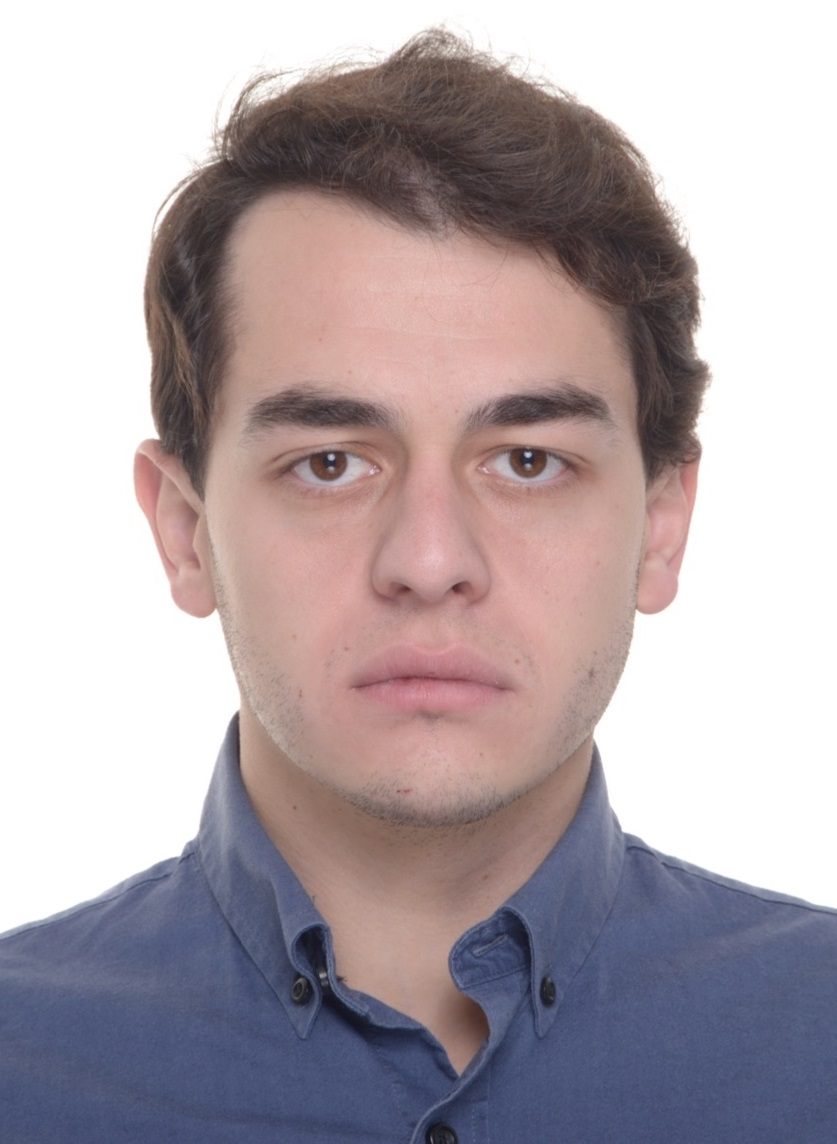
\includegraphics[width=.9\textwidth]{images/bakar.jpg}
		\end{minipage}%
		\hspace{.03\textwidth}%
		\begin{minipage}[b]{.57\textwidth}%
			{\Large\bfseries\thevorname, \thenachname}\\
			\vspace{.5\baselineskip}%
			\thetype\\
			{\scshape\thetitleenglish}\\

			\vspace{\fill}
			\emph{\theadvisorlabel: \thebetreuer}
		\end{minipage}%
		\hspace{.03\textwidth}
	};

	\draw[draw=black!20,line width=1pt] ($(card.north west)+(0,1.2cm)$) to ++(0,-1cm);
	\draw[draw=black!20,line width=1pt] ($(card.north west)+(-1.2cm,0)$) to ++(1cm,0);

	\draw[draw=black!20,line width=1pt] ($(card.north east)+(0,1.2cm)$) to ++(0,-1cm);
	\draw[draw=black!20,line width=1pt] ($(card.north east)+(1.2cm,0)$) to ++(-1cm,0);

	\draw[draw=black!20,line width=1pt] ($(card.south west)+(0,-1.2cm)$) to ++(0,1cm);
	\draw[draw=black!20,line width=1pt] ($(card.south west)+(-1.2cm,0)$) to ++(1cm,0);

	\draw[draw=black!20,line width=1pt] ($(card.south east)+(0,-1.2cm)$) to ++(0,1cm);
	\draw[draw=black!20,line width=1pt] ($(card.south east)+(1.2cm,0)$) to ++(-1cm,0);
\end{tikzpicture}
\vfill
\end{document}
